

\begin{wrapfigure}{r}{4in}
\centering
%\fbox
{ \includegraphics[width=4in,page=2,
trim={11.7cm 0.1cm 27cm 0.1cm},clip
]{diag/2020_NSF_Seda.pdf}}
    \caption{\hlt{Not sure if we need this plot, it we want to, I would like AI people to pick boxes where to assign them}}
 \vskip-10pt    
    \label{fig:managementPlan}
\end{wrapfigure} 
Within the arena of AI and data science, deep learning has emerged as a game-changing technique in recent years with its ability to effectively work on raw big data, bypassing the (otherwise crucial) manual empirical modeling or featurization steps traditionally required for machine learning models. This has enabled numerous real-world applications, such as autonomous driving, machine translation, and visual object recognition. In this proposed institute, we plan to leverage these advances -- both from our team members' prior works and the AI/ML community as a whole -- to enable and establish a gateway for autonomous intelligent physics. We expect to work with multiple physics applications as illustrated earlier, involving a variety of AI challenges, including but not limited to data being too big, too small, high dimensional, high velocity, and so on. Below we briefly describe the proposed AI advances to deal with such challenges in the context of the physics applications described in Section~\ref{sec:physics}. 

\subsubsection{Deeper Learning}
In this era of big data, unsurprisingly the biggest challenges are posed by the large volume, variety, veracity, and velocity of data. One approach to address these challenges is to use large architectures of simple non-linear functions, so-called Deep Neural Networks (DNN), to try to unlock the hidden information contained within the statistical distributions of the data. 
It has been a common trend to build networks deeper and deeper, i.e., more number of hidden layers, in a bid to boost model accuracy. This approach, however, has diminishing returns at best. In fact, arbitrarily making these networks deeper can lead to performance degradation. This is due to the vanishing gradient problem where the gradient or the partial derivative of the loss function w.r.t. the network weights becomes vanishingly small during network training, effectively halting the training. These issues become particularly important for real-time analysis in physics because: i) It is essential to minimize model over-parameterization for resource management; and ii) Models must be extremely data efficient to learn from limited data. Several solutions have been proposed for this issue such as residual learning for image data sets \cite{He_2016_CVPR}, where skip connections are added across a group of stacked convolution layers of the network. Recently, we introduced the concept of individual residual learning for regression tasks on generic tabular data and demonstrated its efficacy for a materials discovery application \cite{Jha_KDD19}. Fig.~\ref{fig:deeperlearning} depicts the performance degradation problem encountered by naively deepening the neural network, and how it can be solved by stacked and individual learning. The individual residual network (IRNet) helped achieve up to 65\% reduction in formation enthalpy prediction error over plain network, and also outperformed traditional ML approaches such as random forest. Unfortunately, most of these advances have not actively permeated specialized scientific domains such as physics yet, and we propose to fill this gap in this AI institute for physics, by creating custom model architectures, neural units, loss functions, and optimization methods to specifically deal with various challenges and resource/latency requirements to enable watershed discoveries in HEP/XRD/EM and physics more broadly. 

\hlt{AA: It would be great if someone could help connect the "HEP/XRD/EM" placeholder in these sections to specific research problems}

\begin{figure*}[tbh]
\centering
  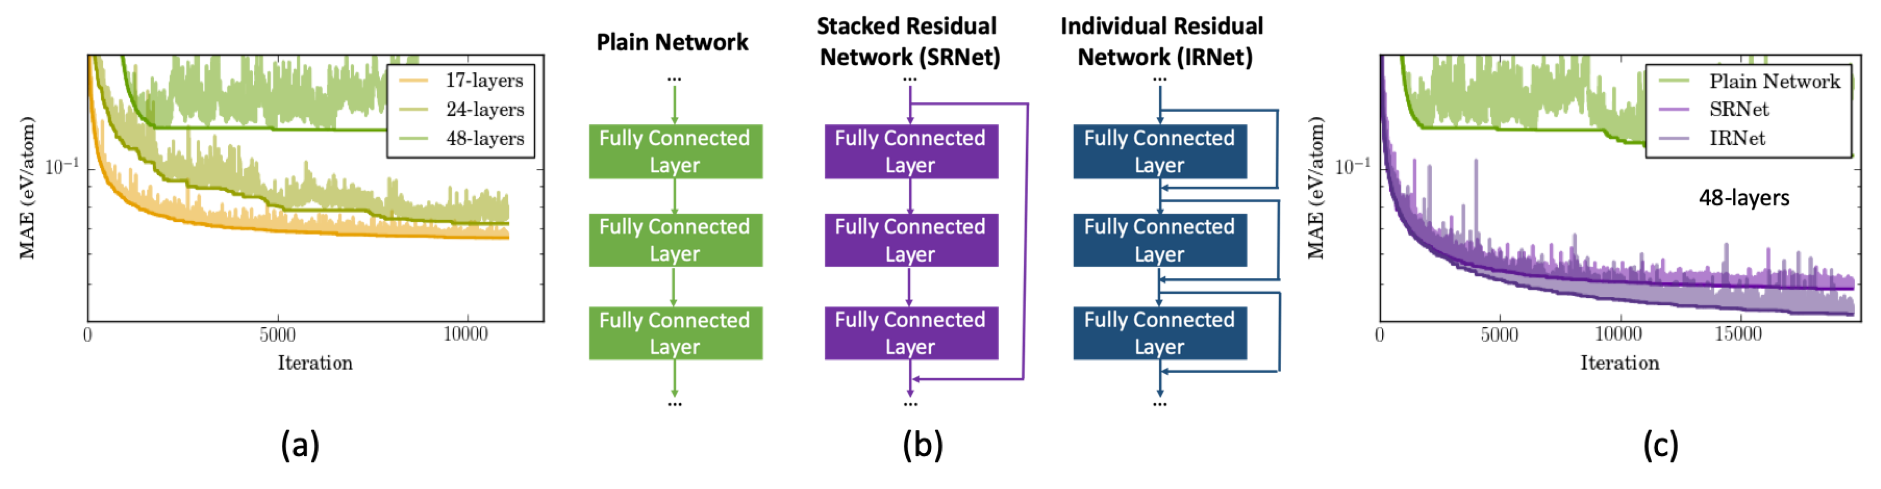
\includegraphics[keepaspectratio, width=\textwidth]{proposal/img/DeeperLearning.png}
  \caption{Illustrative deeper learning using individual residual networks on a materials property prediction dataset \cite{Jha_KDD19}. (a) Learning curves for plain fully connected networks with 17, 24, and 48 layers, depicting the performance degradation problem. (b) Network architectures: plain, stacked residual, and individual residual networks. (c) Learning curves with 48 layer networks with different architectures, depicting superior performance with individual residual learning. In this project, we plan to extend individual residual learning for classification tasks and adapt it for the HEP/XRD/EM data from the application use cases. }
  \label{fig:deeperlearning}
\end{figure*}


\subsubsection{Data Exploration}

 
 
\myparagraph{Transfer Learning.}
One problem with AI/ML models is that they require a large amount of data and computation for training. Fortunately, many common data types can be artificially generated using empirical functions. For example, in EELS spectroscopy data of the similar form can be generated using a summation of Gaussians. This allows us to generate infinite amounts of data which is significantly more complex than the experimental data. While the subsequent learning of a highly over-parameterized unsupervised ML model is not applicable (even after standardization) to experimental data directly, it is possible to use fine-tuning and regularization scheduling to rapidly reduce model complexity and performance simultaneously. \textbf{Co-PIs Choudhary and Agrawal} have applied transfer learning to a variety of tasks including models for crack detection in images \cite{Gopalakrishnan_CBM17}, prediction of wallpaper group symmetry, and ElemNet-based transfer learning to fine-tune the weights of ElemNet \cite{Jha_SciRep18} on smaller data sets yielding highly accurate predictive models even on limited experimental data \cite{Jha_NatComm19}. Transfer learning is able to reduce the distribution divergence such that the models on the target domain can be learned, and have been widely used for anomaly detection, noise detection, even learning from noisy label \cite{aghamaleki2018transfer,lee2018cleannet,andrews2016transfer}.
We will utilize and build upon this experience to design pre-trained networks and transfer learning optimization methods to accelerate discoveries in physics. 

\myparagraph{Physics-Inspired Deep Neural Networks.} \label{physics inspired}
AI algorithms take data in the form of fully-unstructured bits and through computation are optimized toward an objective.
To make AI more efficient it is essential to structure the algorithms in ways that preserve meaningful associations and are equivariant to physically meaningful tensor operations.
For instance, image processing AI use convolutions to consider the Euclidean distance in space and translations equivariant.
Without convolutions, image analysis tasks are less data and computationally efficient. 
Furthermore, to reduce computational complexity, AI algorithms use various forms of compression.
This is most commonly achieved through pooling layers which conduct a down sampling operation.
\todo[inline]{Josh, is this sentence below ok?}
While most of the successful tasks in AI rely on real evenly sampled spatial and temporal domains in physics it is common to acquire data in multiple transformed geometries.
For instance, it is common to collect images composed of the coherent diffraction of high-energy light source or electrons. 
%\hlt{**TODO insert an example for LHC**}
While this data is an image, the physically important information is the position and symmetry of the image, not the arrangement of textures in real space images. In turn, the common process of convolution and pooling discards the most important information. 
In reality the problem is much more complex than just reciprocal space. In physics it is essential to have algorithms that can preserve physically important information.

AI\textsuperscript{3} will facilitate research on approaches which leverage experimental physics knowledge to design efficient AI methods both in terms of data and computational complexity:
\todo[inline]{this should be redone as paragraphs....}
\begin{enumerate}[noitemsep,topsep=0pt]
    \item Symmetry Equivariant Neural Networks
    \hlt{TODO}
    
    \item \todo[inline]{JA} models which will promote periodicity ... (constraints)
\end{enumerate}


\myparagraph{--- creating artificial data --- Josh}
Josh, here we discussed that we could generate some artificial data which could help ML model to warmstart 

\subsubsection{Reinforcement Learning}



\subsubsection{Anomaly Detection}

\subsubsection{Compression and Efficiency}

\hlt{give a brief motivation}


\myparagraph{Data Compression} 


\myparagraph{Architecture Compression} %Tensor Neural Networks
Multi-channel data (e.g. multispectral and hyperspectral imaging) demand more general signal processing schemes than those applied to scalar data. Although the most common arrangement of multi-channel data in physics is in the form of vector signals, there are more complex cases where signal models based on tensor fields are a natural choice.
Tensors, as a generalization of vectors and matrices, provide a natural and concise mathematical framework for formulating and solving problems of this type. \textbf{Co-PI He} has tackled a variety of tasks at tensor-level, such as multi-dimensional data modeling and recognition \cite{he2017kernelized,he2017multi,he2014dusk}, multi-source data aggregation \cite{he2018self,shao2015clustering,lu2018learning,lu2017multilinear}, structured sparse regularization \cite{he2018boosted}, robust streaming tensor factorization and completion \cite{najafi2019outlier} etc. Within AI\textsuperscript{3}, she will explore: 1) building a generic tensor neural architecture that simultaneously addresses many questions in multi-X learning, where X is dimension, view, instance, label, task or part; 2) investigate different types of tensor decompositions both for data compression and accelerating neural architectures, e.g., CANDECOMP/PARAFAC decomposition, Tucker decomposition, tensor train decomposition, etc.; 3) customize the loss function to incorporate physical constraints into a deep tensor neural network architecture for different tasks; 4) explore the attention mechanism to select better attribute features. The need for reliable identification of relevant features in the data is especially important in physics system.

% This goal could be to build a generic tensor neural architecture that simultaneously addresses many questions in multi-X learning, where X is dimension, view, instance, label, task or part. These developments are all based on the notion that related information should be shared to leverage the ...


% \begin{itemize}[noitemsep,topsep=0pt]
    
% %    \item Anomaly  and outlier detection - the goal would be to derive an ML which can automatically flag unusual (rare) behavior (e.g., if the rare events are what we are aiming to pick, then one can use e.g., autoencoders to do the job); 
%         \item facilitate characterization by generating intelligent data that provides actionable information in real-time
%     \item Data Representation: 
%     strength of statistics. 
%     \item Data-efficient learning: for example: X-ray microscopy yields limited data per limited amount of time
%     %\item Physics-inspired deep neural networks (DNN) - this goal could be to utilize some basic understanding of the domain knowledge to formulate the deep neural network to capture the physical understanding of the world
%     \item 
% Incorporating physical laws into DNN models - I am not sure if this would be particularly useful, but one can aim to enforce some physical laws to be satisfied by the ML models.  (non-negativity constraints, box constraints for domain...)
% \end{itemize} 






\subsubsection{Explainable AI}
Explainable AI is a set of tools and frameworks to help develop interpretable and inclusive AI models and deploy them with confidence. We propose to leverage representation learning and model explainability in the following forms to help bring AI models to a broader and confident applications in physics.

\myparagraph{Representation Learning.} The primary goal in experimental physics is to turn data into actionable information. One way AI can facilitate this is by learning meaningful representations in the forms of structured latent manifolds. In preparation of this proposal \textbf{co-PI Agar} conducted preliminary studies applying an unsupervised sparse long-short term memory (LSTM) autoencoder developed for analysis of multi-dimensional scanning probe spectroscopy to atomically resolved EELS of an LaSrMnO\textsubscript{3}. Briefly, a sparse LSTM-autoencoder was trained on the EELS spectra \hlt{(TODO ADD Figure)}\cite{agar_revealing_2019}. Following training, we visualized the learned information by computing the output of the sparse low-dimensional embedding layer to form real-space feature maps. These feature maps were able to automatically identify the most important physically significant characteristics of the interface. This result means that the autoencoder is capable of learning a complex identity function where each neuron controls a physically meaningful characteristic of the response. Furthermore, the autoencoder is also able to quantify the relative response character (i.e., how “x-like” the response is). This deviates from approaches that generally provide the only classification of behavior (i.e., belong to group “x”) or have linear latent spaces. The autoencoder is also able to interpret the latent space by using it as a generator to visualize what x encodes.
Particularly interesting is the ability of this approach to quantify the electronic sharpness of the interface, a difficult to measure property that strongly influences correlated electron effects at interfaces (e.g., 2-dimensional electron gases). 
%Learning accurate, concise, and meaningful data representation is the key to most AI/ML tasks, and this is even more true for scientific and engineering applications. We propose to design and develop DNN models to learn latent representations of the scientific data from physics applications in this project. 
As another example, \textbf{co-PIs Choudhary and Agrawal} recently developed a DNN called ElemNet \cite{Jha_SciRep18} that uses only raw elemental compositions to predict inorganic materials properties. Although no periodic table information was provided to the model, it could self-learn interesting chemistry knowledge, such as element similarity (groups in the periodic table) and charge balance (element interaction) and could also predict phase diagrams on unseen systems. 

AI\textsuperscript{3} will facilitate a coordinated effort amongst \textbf{co-Pis Agar, Choudhary, Agrawal, and He} to extend these works to learn interpretable and meaningful representations of HEP/XRD/EM data, which could subsequently be used to derive application specific models. We will also investigate the impact of different data representation learning techniques, by exploring fundamental AI concepts to help learn and shape learned latent representations. Potential research areas to explore are controlled variationality,  regularization and regularization scheduling during training (e.g., L\textsubscript{2}\xrightarrow{}L\textsubscript{p}, \ $p \in (0,2)$), fine-grained representations from learning with attention mechanism, Bayesian representations and uncertainty predictions  and adversarial autoencoders.   

\myparagraph{Model Explanation.} \hlt{--- add text --- Su}

% \subsubsection{Efficient AI Algorithms}
% \color{orange} N.T.: Do we need another category on building more efficient ``core AI'' algorithms?
% \color{black}
% \begin{itemize}[noitemsep,topsep=0pt]
%     \item 
    
% }
    
%     reduced precision
%     \hlt{***there are some papers where they even try to do precision automatically based on the weights -- different layers can have different precision***}
%     \item pruning/compression
%     \item architecture portability (related to transfer learning)
%     \item more efficient structures with physics built in (related to ``physics-inspired section'')
% \end{itemize}



%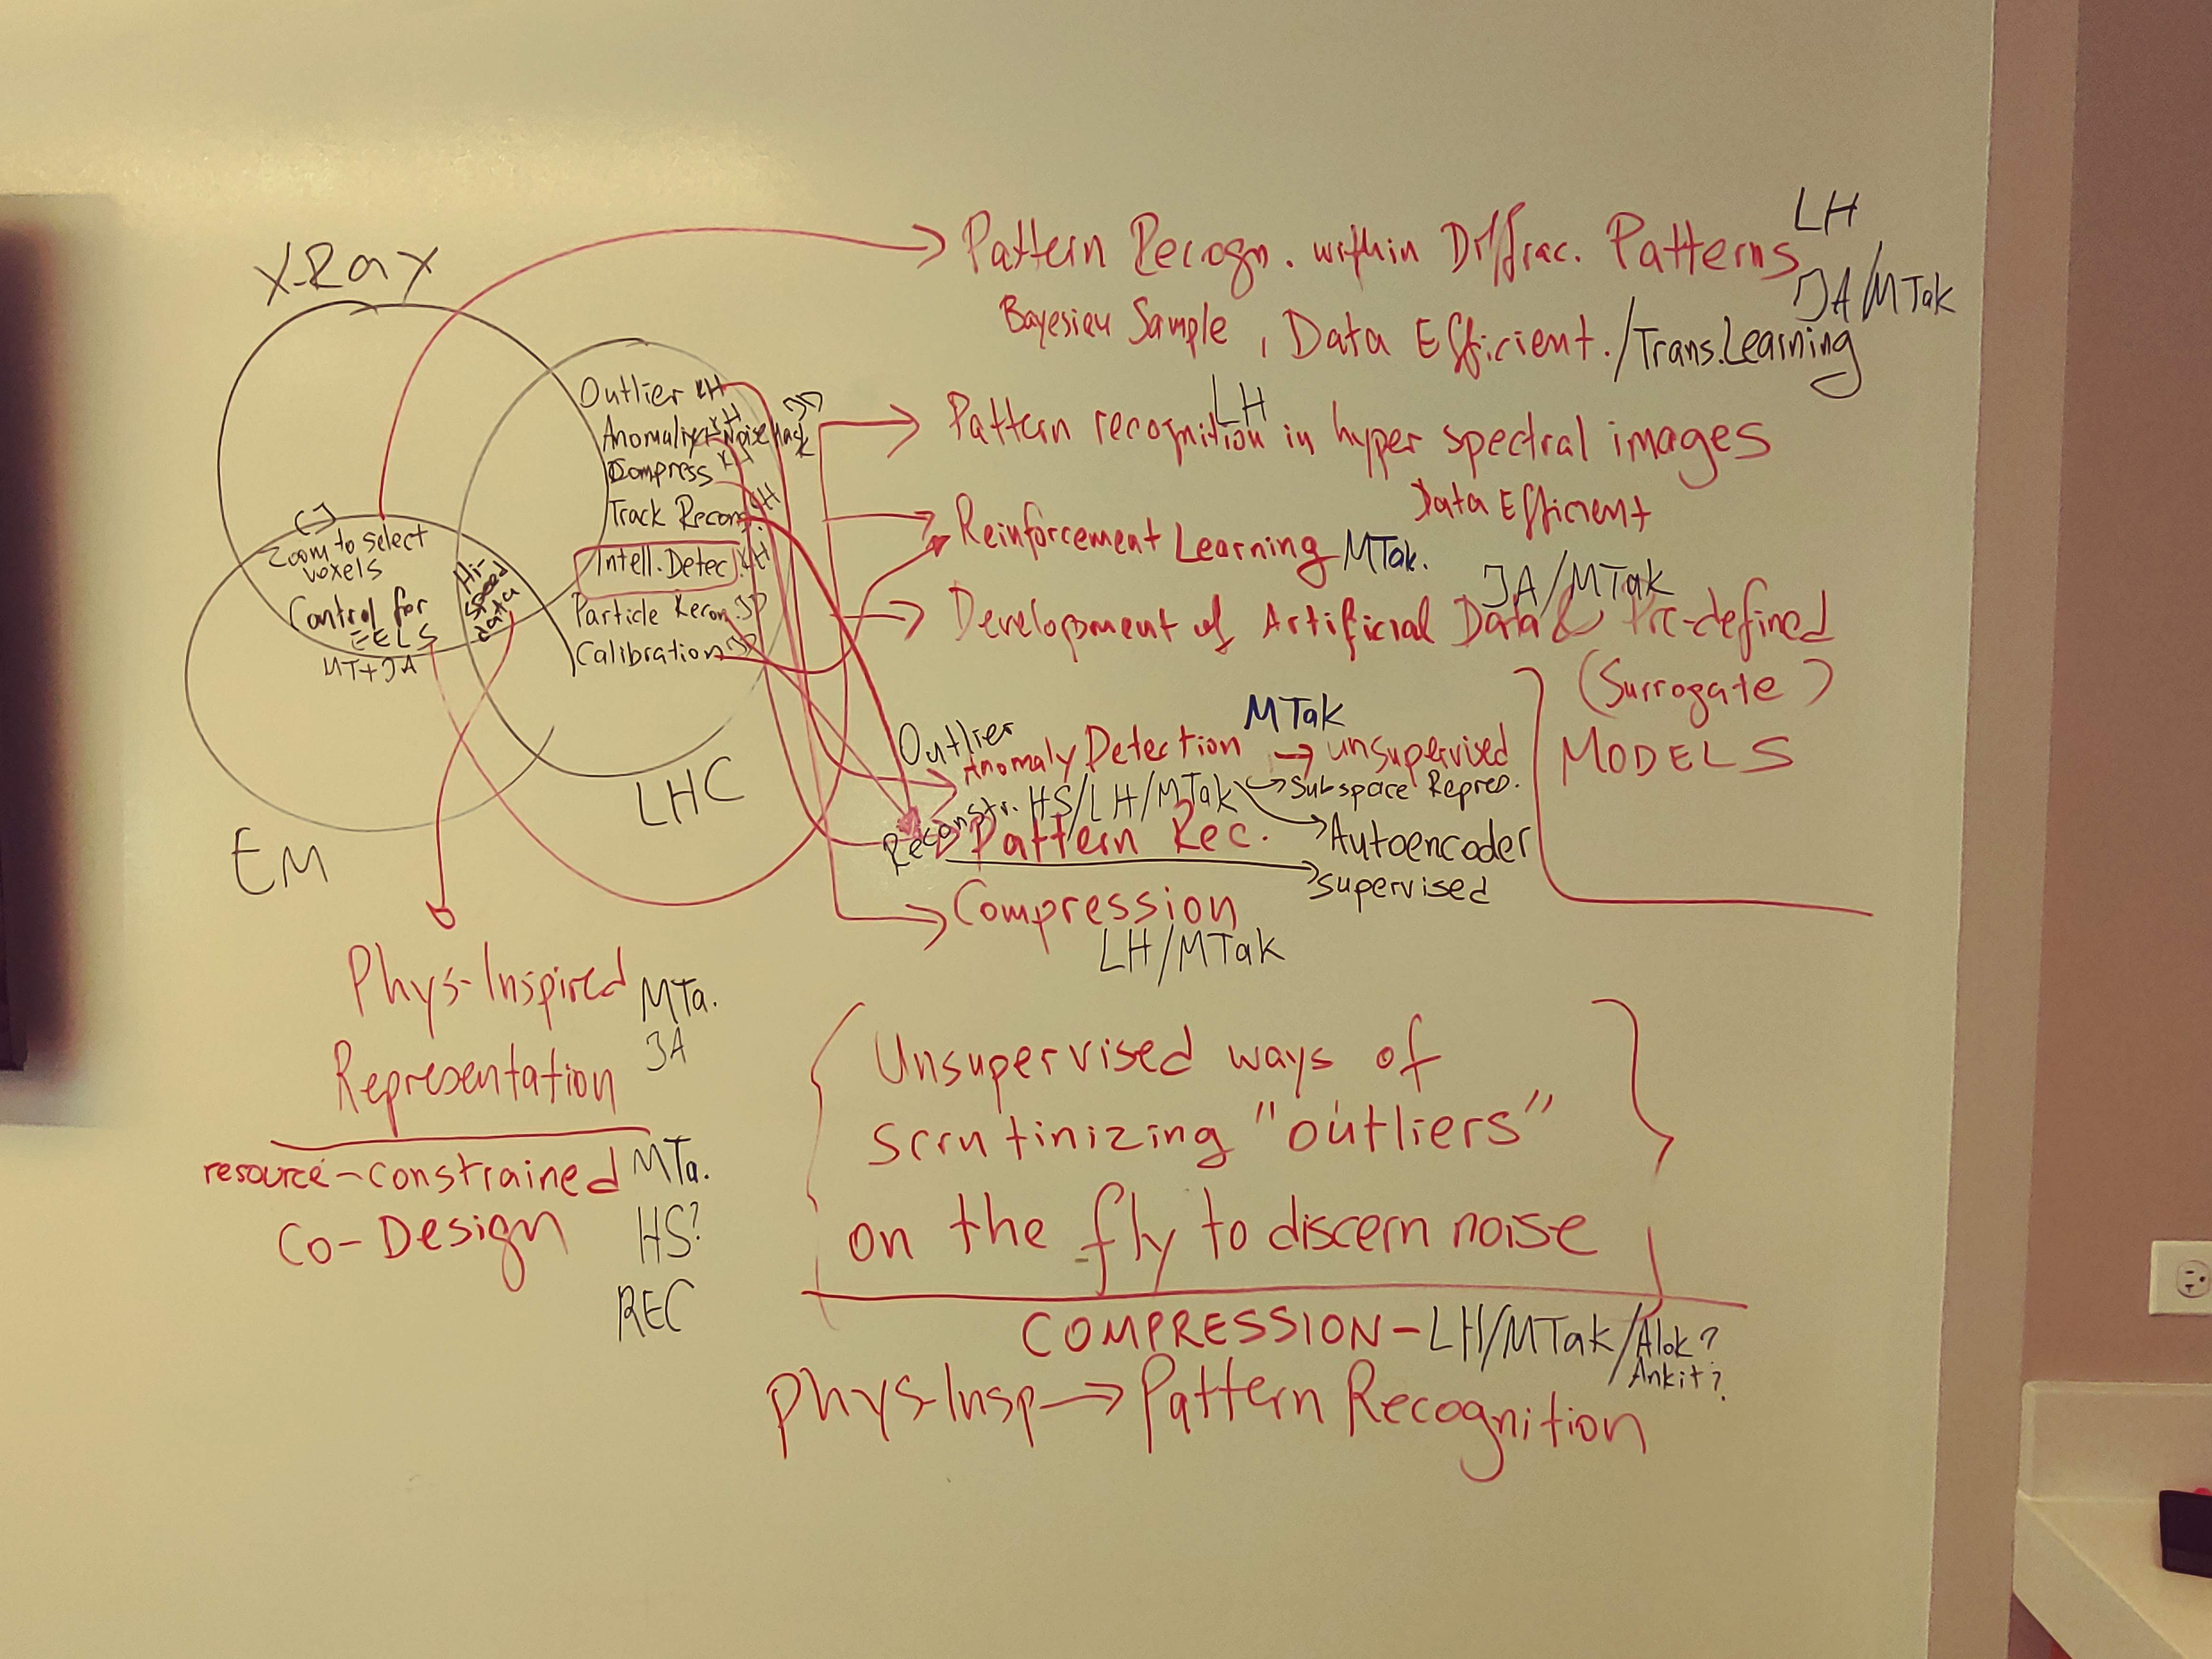
\includegraphics[width=8in]{20200102_133731.jpg}

 